% blog-title: Concentration Bounds in Bandit Analysis
% blog-date: 2026-06-18
% blog-description: A polished note on how Hoeffding, Bernstein, and sub-Gaussian tails become error bars, UCB indices, and regret-control tools.
% blog-lang: en

\documentclass[en,nofont,11pt]{elegantbook}

\title{Concentration Bounds in Bandit Analysis}
\subtitle{Hoeffding, Bernstein, and Sub-Gaussian Tails}
\author{Tang}
\institute{Tang's Machine Learning Blog}
\date{2026-06-18}
\version{1.0.0}
\bioinfo{Topic}{Concentration Bounds, UCB, Bandit Analysis}
\cover{assets/blog-cover.jpg}

\usepackage{fontspec}
\ifdefined\setCJKmainfont
\else
  \usepackage[UTF8,scheme=plain,fontset=none]{ctex}
\fi
\usepackage{xcolor}
\usepackage{listings}
\usepackage{float}
\usepackage{tcolorbox}
\tcbuselibrary{breakable, listings, skins}
\usetikzlibrary{arrows.meta,positioning,calc,decorations.pathmorphing,decorations.pathreplacing,fit,backgrounds,patterns,shapes.geometric}

\IfFontExistsTF{Microsoft YaHei}{
  \setCJKmainfont{Microsoft YaHei}
  \setCJKsansfont{Microsoft YaHei}
  \setCJKmonofont{Microsoft YaHei UI}
}{
  \IfFontExistsTF{Noto Serif CJK SC}{
    \setCJKmainfont{Noto Serif CJK SC}
    \setCJKsansfont{Noto Sans CJK SC}
    \setCJKmonofont{Noto Sans Mono CJK SC}
  }{}
}

\definecolor{blogAccent}{HTML}{1F6F8B}
\definecolor{blogInk}{HTML}{172026}
\definecolor{blogCodeBg}{HTML}{F5F7F8}
\definecolor{blogCodeBorder}{HTML}{D6E2E8}
\definecolor{blogKeyword}{HTML}{B23A48}
\definecolor{blogString}{HTML}{287D4F}
\definecolor{blogComment}{HTML}{687783}

\lstdefinestyle{blogcode}{
  basicstyle=\ttfamily\small,
  keywordstyle=\bfseries\color{blogKeyword},
  stringstyle=\color{blogString},
  commentstyle=\itshape\color{blogComment},
  numberstyle=\scriptsize\color{blogComment},
  numbers=left,
  numbersep=8pt,
  showstringspaces=false,
  breaklines=true,
  tabsize=2,
  columns=fullflexible,
  keepspaces=true
}

\newtcblisting{codeblock}[2][]{
  listing only,
  breakable,
  enhanced,
  colback=blogCodeBg,
  colframe=blogCodeBorder,
  arc=2mm,
  boxrule=0.4pt,
  left=6mm,
  right=2mm,
  top=1mm,
  bottom=1mm,
  listing options={style=blogcode, language=#2},
  #1
}

\hypersetup{
  colorlinks=true,
  linkcolor=blogAccent,
  urlcolor=blogAccent,
  citecolor=blogAccent
}

\addbibresource{tex/bandits-references.bib}

\definecolor{concentrationBlue}{RGB}{28,73,135}
\definecolor{concentrationLightBlue}{RGB}{232,241,252}
\definecolor{concentrationOrange}{RGB}{150,75,25}
\definecolor{concentrationLightOrange}{RGB}{255,247,236}
\definecolor{concentrationGray}{RGB}{247,247,247}
\colorlet{mainblue}{concentrationBlue}
\colorlet{lightblue}{concentrationLightBlue}
\colorlet{deeporange}{concentrationOrange}
\colorlet{lightorange}{concentrationLightOrange}
\colorlet{lightgray}{concentrationGray}

\newtcolorbox{keyidea}[1][]{enhanced,breakable,colback=lightblue,colframe=mainblue,
  coltitle=white,fonttitle=\bfseries,title=Key idea,#1}
\newtcolorbox{thinkbox}[1][]{enhanced,breakable,colback=lightorange,colframe=deeporange,
  coltitle=white,fonttitle=\bfseries,title=Think,#1}
\newtcolorbox{resultbox}[1][]{enhanced,breakable,colback=white,colframe=mainblue,
  coltitle=white,fonttitle=\bfseries,title=Result,#1}

\newcommand{\E}{\mathbb{E}}
\newcommand{\Pbb}{\mathbb{P}}
\newcommand{\R}{\mathbb{R}}
\newcommand{\one}{\mathbf{1}}
\newcommand{\Var}{\operatorname{Var}}
\newcommand{\KL}{\operatorname{KL}}
\newcommand{\argmax}{\operatorname*{arg\,max}}

\begin{document}
\maketitle
\frontmatter
\tableofcontents
\mainmatter

\chapter{The Error Bar Is the Algorithm}

A bandit algorithm looks like a decision rule. It chooses an arm. It receives a reward. It chooses again. But inside almost every clean bandit proof there is a smaller object doing most of the work: an error bar.

If the empirical mean of an arm is the number we can see, the true mean is the number we want. The distance between them is invisible. Concentration inequalities are the tools that make this invisible distance usable.

\begin{keyidea}
A concentration bound is not just a probability lemma. In bandit theory it becomes an algorithmic object. It tells the learner how much optimism is still defensible after seeing a certain amount of data.
\end{keyidea}

The whole story of UCB can be read as one sentence:
\[
\text{choose the arm with the largest plausible mean.}
\]
The word ``plausible'' is where probability enters.

\section{A small picture}

Consider four actions. Each has an unknown click probability. The learner sees only the reward of the action it chose.

\begin{center}
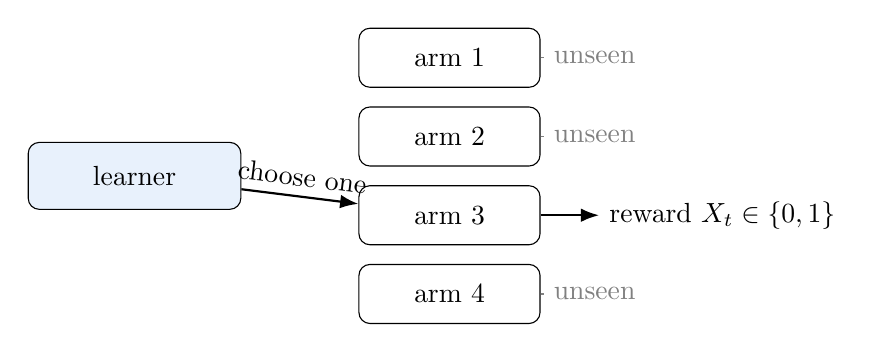
\begin{tikzpicture}[>=Latex,scale=1]
\node[draw,rounded corners,fill=lightblue,minimum width=2.7cm,minimum height=0.85cm] (learner) at (0,0) {learner};
\node[draw,rounded corners,fill=white,minimum width=2.3cm,minimum height=0.75cm] (a1) at (4,1.5) {arm 1};
\node[draw,rounded corners,fill=white,minimum width=2.3cm,minimum height=0.75cm] (a2) at (4,0.5) {arm 2};
\node[draw,rounded corners,fill=white,minimum width=2.3cm,minimum height=0.75cm] (a3) at (4,-0.5) {arm 3};
\node[draw,rounded corners,fill=white,minimum width=2.3cm,minimum height=0.75cm] (a4) at (4,-1.5) {arm 4};
\draw[->,thick] (learner) -- node[above,sloped]{choose one} (a3);
\draw[->,thick] (a3) -- ++(1.9,0) node[right]{reward $X_t\in\{0,1\}$};
\draw[dashed,gray] (a1) -- ++(1.2,0) node[right,gray]{unseen};
\draw[dashed,gray] (a2) -- ++(1.2,0) node[right,gray]{unseen};
\draw[dashed,gray] (a4) -- ++(1.2,0) node[right,gray]{unseen};
\end{tikzpicture}
\end{center}

The hard part is not that rewards are random. The hard part is that the data are produced by our past decisions. If an arm looks bad early, we may stop sampling it. If it looks good early, we may sample it more. The sample size of each arm is itself a random outcome of the algorithm.

This is why concentration in bandits must be slightly more careful than concentration in a fixed dataset.

\chapter{One Random Number, Then Many}

We start from the smallest possible object.

A random variable is a number we do not know yet. If $X$ is a Bernoulli reward, then
\[
X =
\begin{cases}
1, & \text{click or success},\\
0, & \text{no click or failure}.
\end{cases}
\]
Its mean is
\[
\mu = \E[X].
\]
For a Bernoulli random variable with success probability $p$,
\[
\E[X]
= 1\cdot p + 0\cdot (1-p)
= p.
\]

Now suppose we pull the same arm $n$ times and obtain
\[
X_1,X_2,\ldots,X_n.
\]
The empirical mean is
\[
\widehat\mu_n = \frac{1}{n}\sum_{i=1}^{n}X_i.
\]
It is the most natural estimate of $\mu$ because
\[
\E[\widehat\mu_n]
= \E\left[\frac{1}{n}\sum_{i=1}^{n}X_i\right]
= \frac{1}{n}\sum_{i=1}^{n}\E[X_i]
= \frac{1}{n}\cdot n\mu
= \mu.
\]

\begin{thinkbox}
The sample mean is unbiased, but unbiased does not mean correct. It means it is right on average over repeated worlds. In one actual run, it can still be too high or too low. Concentration asks: by how much?
\end{thinkbox}

\section{The event we care about}

The basic bad event is
\[
\left\{\widehat\mu_n - \mu \ge r\right\}.
\]
This event says: the empirical mean is too optimistic by at least $r$.

The two-sided bad event is
\[
\left\{|\widehat\mu_n - \mu| \ge r\right\}
= \left\{\widehat\mu_n - \mu \ge r\right\}
\cup
\left\{\mu - \widehat\mu_n \ge r\right\}.
\]
Therefore
\[
\Pbb\!\left(|\widehat\mu_n - \mu| \ge r\right)
\le
\Pbb\!\left(\widehat\mu_n - \mu \ge r\right)
+
\Pbb\!\left(\mu - \widehat\mu_n \ge r\right).
\]
This is the union bound. It says that if either of two things can go wrong, the chance that something goes wrong is at most the sum of the two chances.

\chapter{Hoeffding: The First Error Bar}

Hoeffding's inequality is the first concentration bound one should learn for bandits. It is simple, robust, and often good enough.

\begin{resultbox}
Let $X_1,\ldots,X_n$ be independent random variables in $[0,1]$ with common mean $\mu$. Then for every $r>0$,
\[
\Pbb\!\left(\widehat\mu_n-\mu\ge r\right) \le \exp(-2nr^2),
\]
and
\[
\Pbb\!\left(|\widehat\mu_n-\mu|\ge r\right) \le 2\exp(-2nr^2).
\]
\end{resultbox}

The statement says that the probability of a large error decays exponentially in $nr^2$. More data makes the error smaller. A larger error is less likely.

\section{The proof idea in one line}

A probability of a large deviation is hard to bound directly. Hoeffding's proof turns the deviation into an exponential moment:
\[
\Pbb(S_n\ge nr)
\quad\longrightarrow\quad
\E[\exp(\lambda S_n)],
\]
where
\[
S_n = \sum_{i=1}^n (X_i-\mu).
\]
The exponential function is useful because products appear when independent variables are added.

\section{Step-by-step proof}

Let
\[
S_n = \sum_{i=1}^{n}(X_i-\mu).
\]
Then
\[
\widehat\mu_n-\mu
= \frac{1}{n}\sum_{i=1}^{n}(X_i-\mu)
= \frac{S_n}{n}.
\]
Hence
\[
\left\{\widehat\mu_n-\mu\ge r\right\}
= \left\{S_n\ge nr\right\}.
\]
For any $\lambda>0$,
\[
S_n\ge nr
\quad\Longleftrightarrow\quad
\exp(\lambda S_n)\ge \exp(\lambda nr).
\]
By Markov's inequality,
\[
\Pbb\!\left(\exp(\lambda S_n)\ge \exp(\lambda nr)\right)
\le
\frac{\E[\exp(\lambda S_n)]}{\exp(\lambda nr)}.
\]
Therefore
\[
\Pbb(S_n\ge nr)
\le
\exp(-\lambda nr)\E[\exp(\lambda S_n)].
\]
Now expand $S_n$:
\[
\E[\exp(\lambda S_n)]
= \E\left[\exp\left(\lambda\sum_{i=1}^{n}(X_i-\mu)\right)\right].
\]
Since the exponential of a sum is a product,
\[
= \E\left[\prod_{i=1}^{n}\exp\left(\lambda(X_i-\mu)\right)\right].
\]
Since $X_i$ are independent,
\[
= \prod_{i=1}^{n}\E\left[\exp\left(\lambda(X_i-\mu)\right)\right].
\]
Hoeffding's lemma for a centered random variable in an interval of length $1$ gives
\[
\E\left[\exp\left(\lambda(X_i-\mu)\right)\right]
\le \exp\left(\frac{\lambda^2}{8}\right).
\]
Thus
\[
\E[\exp(\lambda S_n)]
\le
\prod_{i=1}^{n}\exp\left(\frac{\lambda^2}{8}\right)
= \exp\left(\frac{n\lambda^2}{8}\right).
\]
Putting this back into the probability bound,
\[
\Pbb(S_n\ge nr)
\le
\exp(-\lambda nr)\exp\left(\frac{n\lambda^2}{8}\right)
= \exp\left(-\lambda nr+\frac{n\lambda^2}{8}\right).
\]
This is true for every $\lambda>0$. We choose the best $\lambda$.

Let
\[
\phi(\lambda)=-\lambda nr+\frac{n\lambda^2}{8}.
\]
Then
\[
\phi'(\lambda)=-nr+\frac{n\lambda}{4}.
\]
Set $\phi'(\lambda)=0$:
\[
-nr+\frac{n\lambda}{4}=0
\quad\Longrightarrow\quad
\lambda=4r.
\]
Substitute $\lambda=4r$:
\[
\phi(4r)=-(4r)nr+\frac{n(4r)^2}{8}
= -4nr^2+\frac{16nr^2}{8}
= -4nr^2+2nr^2
= -2nr^2.
\]
Therefore
\[
\Pbb(\widehat\mu_n-\mu\ge r)
= \Pbb(S_n\ge nr)
\le \exp(-2nr^2).
\]
The same argument applied to $-S_n$ gives
\[
\Pbb(\mu-\widehat\mu_n\ge r)
\le \exp(-2nr^2).
\]
Finally,
\[
\Pbb(|\widehat\mu_n-\mu|\ge r)
\le
\exp(-2nr^2)+\exp(-2nr^2)
=2\exp(-2nr^2).
\]

\begin{keyidea}
Hoeffding turns ``the sample mean might be wrong'' into a number. That number is an error bar.
\end{keyidea}

\chapter{From Tail Bound to Confidence Radius}

The inequality
\[
\Pbb(|\widehat\mu_n-\mu|\ge r)
\le 2\exp(-2nr^2)
\]
is not yet an algorithm. An algorithm needs a radius $r$.

Choose a failure probability $\delta\in(0,1)$. We want
\[
2\exp(-2nr^2)\le \delta.
\]
Now solve for $r$ step by step:
\[
2\exp(-2nr^2)\le \delta,
\]
\[
\exp(-2nr^2)\le \frac{\delta}{2},
\]
\[
-2nr^2 \le \log\left(\frac{\delta}{2}\right),
\]
\[
2nr^2 \ge \log\left(\frac{2}{\delta}\right),
\]
\[
r^2 \ge \frac{\log(2/\delta)}{2n},
\]
\[
r \ge \sqrt{\frac{\log(2/\delta)}{2n}}.
\]
Therefore the Hoeffding confidence radius is
\[
\boxed{
\operatorname{rad}_{\rm H}(n,\delta)
=\sqrt{\frac{\log(2/\delta)}{2n}}.
}
\]
With probability at least $1-\delta$,
\[
\mu\in
\left[
\widehat\mu_n-\operatorname{rad}_{\rm H}(n,\delta),
\widehat\mu_n+\operatorname{rad}_{\rm H}(n,\delta)
\right].
\]

\begin{thinkbox}
Do not remember only the formula. Remember the tradeoff: the radius shrinks like $1/\sqrt n$ and grows like $\sqrt{\log(1/\delta)}$. Confidence is not free. Asking for a very small failure probability makes the interval wider.
\end{thinkbox}

\chapter{Why Bandits Need Many Error Bars at Once}

In supervised learning, one often analyzes a fixed estimator at a fixed sample size. In bandits, the learner keeps looking, choosing, and updating. At time $t$, each arm $a$ has its own random number of pulls
\[
N_a(t)=\sum_{s=1}^{t}\one\{A_s=a\}.
\]
The sample mean of arm $a$ is
\[
\widehat\mu_a(t)
=\frac{1}{N_a(t)}\sum_{s=1}^{t}\one\{A_s=a\}X_s,
\]
when $N_a(t)>0$.

The learner wants all confidence intervals to be correct at all relevant times. A simple way to do this is to buy many error bars with one failure budget.

Suppose there are $K$ arms and $T$ rounds. There are at most $KT$ arm-time pairs. Give each pair failure probability
\[
\delta' = \frac{\delta}{KT}.
\]
For one pair $(a,t)$, Hoeffding gives
\[
\Pbb\left(
|\widehat\mu_a(t)-\mu_a|
>
\sqrt{\frac{\log(2/\delta')}{2N_a(t)}}
\right)
\le \delta'.
\]
By the union bound,
\[
\Pbb\left(\text{at least one arm-time interval fails}\right)
\le
\sum_{a=1}^{K}\sum_{t=1}^{T}\delta'
=KT\cdot \frac{\delta}{KT}
=\delta.
\]
Thus, with probability at least $1-\delta$, every displayed error bar is correct.

\begin{keyidea}
The union bound is not a crude technicality here. It is the mechanism that lets an adaptive algorithm look at many arms many times without pretending that each look is isolated.
\end{keyidea}

\chapter{UCB from Hoeffding}

For arm $a$, define the optimistic index
\[
U_a(t)=\widehat\mu_a(t)+\sqrt{\frac{2\log t}{N_a(t)}}.
\]
The exact constant is not sacred. The structure is sacred:
\[
\text{index} = \text{what we have seen} + \text{how wrong it could still be}.
\]
At each round,
\[
A_t\in \argmax_{a\in[K]} U_a(t).
\]

\section{Algorithm design}

\begin{codeblock}[title={Hoeffding-UCB core rule.}]{Python}
def ucb_hoeffding_action(t, sums, counts):
    means = sums / counts
    bonus = np.sqrt(2.0 * np.log(t + 1.0) / counts)
    return int(np.argmax(means + bonus))
\end{codeblock}

The code is short because the theorem is doing the work. The square-root term is the confidence radius.

\section{The standard pull-count calculation}

Let $a^*$ be an optimal arm and let
\[
\Delta_a=\mu_{a^*}-\mu_a>0
\]
for a suboptimal arm $a$.

On a good event, all confidence intervals are correct. For every arm $b$ and time $t$,
\[
|\widehat\mu_b(t)-\mu_b|
\le
\sqrt{\frac{2\log t}{N_b(t)}}.
\]
If UCB chooses a suboptimal arm $a$ at time $t$, then
\[
U_a(t)\ge U_{a^*}(t).
\]
Since the optimal arm's index is optimistic,
\[
U_{a^*}(t)
=\widehat\mu_{a^*}(t)+\sqrt{\frac{2\log t}{N_{a^*}(t)}}
\ge \mu_{a^*}.
\]
Therefore
\[
U_a(t)\ge \mu_{a^*}.
\]
But on the good event,
\[
\widehat\mu_a(t)\le \mu_a+\sqrt{\frac{2\log t}{N_a(t)}}.
\]
Hence
\[
U_a(t)
=\widehat\mu_a(t)+\sqrt{\frac{2\log t}{N_a(t)}}
\le
\mu_a+2\sqrt{\frac{2\log t}{N_a(t)}}.
\]
Combining the lower and upper bounds on $U_a(t)$,
\[
\mu_{a^*}
\le
\mu_a+2\sqrt{\frac{2\log t}{N_a(t)}}.
\]
Subtract $\mu_a$:
\[
\Delta_a
\le
2\sqrt{\frac{2\log t}{N_a(t)}}.
\]
Divide by $2$:
\[
\frac{\Delta_a}{2}
\le
\sqrt{\frac{2\log t}{N_a(t)}}.
\]
Square both sides:
\[
\frac{\Delta_a^2}{4}
\le
\frac{2\log t}{N_a(t)}.
\]
Rearrange:
\[
N_a(t)
\le
\frac{8\log t}{\Delta_a^2}.
\]
Thus a suboptimal arm can be pulled many times only if its uncertainty is still large. Once it has been sampled enough, optimism can no longer hide its gap.

The regret contribution of arm $a$ is approximately
\[
\Delta_a \E[N_a(T)].
\]
The calculation above explains the familiar logarithmic shape:
\[
\Delta_a N_a(T)
\lesssim
\Delta_a\cdot \frac{8\log T}{\Delta_a^2}
=
\frac{8\log T}{\Delta_a}.
\]

\chapter{Bernstein: When Variance Matters}

Hoeffding only uses the fact that rewards lie in $[0,1]$. It does not ask whether the arm is noisy or nearly deterministic.

But this matters. A Bernoulli arm with mean $0.5$ has variance
\[
0.5(1-0.5)=0.25.
\]
A Bernoulli arm with mean $0.05$ has variance
\[
0.05(1-0.05)=0.0475.
\]
Both rewards lie in $[0,1]$, but the second one fluctuates much less.

Bernstein-type bounds use this variance information.

\begin{resultbox}
A simple Bernstein-style confidence radius has the form
\[
\operatorname{rad}_{\rm B}(n,\delta,\sigma^2)
=
\sqrt{\frac{2\sigma^2\log(2/\delta)}{n}}
+
\frac{\log(2/\delta)}{3n}.
\]
The first term is variance-sensitive. The second term is a boundedness correction.
\end{resultbox}

\section{How to read the formula}

Compare Hoeffding and Bernstein:
\[
\operatorname{rad}_{\rm H}(n,\delta)
=\sqrt{\frac{\log(2/\delta)}{2n}},
\]
\[
\operatorname{rad}_{\rm B}(n,\delta,\sigma^2)
=\sqrt{\frac{2\sigma^2\log(2/\delta)}{n}}
+\frac{\log(2/\delta)}{3n}.
\]
If $\sigma^2$ is small, the square-root term is small. For large $n$, the $1/n$ correction becomes smaller than the $1/\sqrt n$ term, and the variance advantage becomes visible.

\begin{figure}[H]
\centering

\includegraphics[width=0.78\linewidth]{assets/concentration/confidence_radius_widths.pdf}
\caption{For a low-variance Bernoulli arm with $p=0.05$, a variance-aware radius can be substantially shorter than Hoeffding's radius.}
\end{figure}

\section{Empirical Bernstein UCB}

In a bandit problem, $\sigma_a^2$ is usually unknown. We estimate it.

For arm $a$, define
\[
\widehat\sigma_a^2(t)
=\frac{1}{N_a(t)}\sum_{s:A_s=a}\left(X_s-\widehat\mu_a(t)\right)^2.
\]
Then an empirical Bernstein-style index is
\[
U_a^{\rm EB}(t)
=\widehat\mu_a(t)
+
\sqrt{\frac{2\widehat\sigma_a^2(t)\log t}{N_a(t)}}
+
\frac{3\log t}{N_a(t)}.
\]

\begin{codeblock}[title={Empirical-Bernstein UCB core rule.}]{Python}
def ucb_bernstein_action(t, sums, sq_sums, counts):
    means = sums / counts
    variances = np.maximum(0.0, sq_sums / counts - means * means)
    log_term = np.log(t + 1.0)
    bonus = np.sqrt(2.0 * variances * log_term / counts) + 3.0 * log_term / counts
    return int(np.argmax(means + bonus))
\end{codeblock}

This is the same design pattern as UCB-Hoeffding, but the error bar now listens to the observed variance.

\chapter{Sub-Gaussian Tails: A Cleaner Language}

Hoeffding is excellent for bounded variables. But many models are not naturally bounded. A Gaussian reward, for example, can take any real value.

A random variable $X$ with mean $\mu$ is called $\sigma$-sub-Gaussian if, for every $\lambda\in\R$,
\[
\E\left[\exp\left(\lambda(X-\mu)\right)\right]
\le
\exp\left(\frac{\lambda^2\sigma^2}{2}\right).
\]

This definition says: the exponential moments of $X-\mu$ are no larger than those of a Gaussian with variance proxy $\sigma^2$.

\section{Tail bound from the definition}

Let $X_1,\ldots,X_n$ be independent $\sigma$-sub-Gaussian random variables with mean $\mu$. Let
\[
\widehat\mu_n=\frac{1}{n}\sum_{i=1}^{n}X_i.
\]
We derive a one-sided tail bound.

Set
\[
S_n=\sum_{i=1}^{n}(X_i-\mu).
\]
Then
\[
\widehat\mu_n-\mu=\frac{S_n}{n}.
\]
For $\lambda>0$,
\[
\Pbb(\widehat\mu_n-\mu\ge r)
=\Pbb(S_n\ge nr)
\]
\[
=\Pbb(\exp(\lambda S_n)\ge \exp(\lambda nr)).
\]
By Markov's inequality,
\[
\Pbb(S_n\ge nr)
\le
\exp(-\lambda nr)\E[\exp(\lambda S_n)].
\]
By independence,
\[
\E[\exp(\lambda S_n)]
=\prod_{i=1}^{n}\E[\exp(\lambda(X_i-\mu))].
\]
By sub-Gaussianity,
\[
\le
\prod_{i=1}^{n}\exp\left(\frac{\lambda^2\sigma^2}{2}\right)
=
\exp\left(\frac{n\lambda^2\sigma^2}{2}\right).
\]
Therefore
\[
\Pbb(\widehat\mu_n-\mu\ge r)
\le
\exp\left(-\lambda nr+\frac{n\lambda^2\sigma^2}{2}\right).
\]
Choose the best $\lambda$.

Let
\[
\psi(\lambda)=-\lambda nr+\frac{n\lambda^2\sigma^2}{2}.
\]
Then
\[
\psi'(\lambda)=-nr+n\lambda\sigma^2.
\]
Set $\psi'(\lambda)=0$:
\[
-nr+n\lambda\sigma^2=0
\quad\Longrightarrow\quad
\lambda=\frac{r}{\sigma^2}.
\]
Substitute:
\[
\psi\left(\frac{r}{\sigma^2}\right)
= -\frac{r}{\sigma^2}nr
+\frac{n}{2}\frac{r^2}{\sigma^4}\sigma^2
= -\frac{nr^2}{\sigma^2}+\frac{nr^2}{2\sigma^2}
= -\frac{nr^2}{2\sigma^2}.
\]
Thus
\[
\Pbb(\widehat\mu_n-\mu\ge r)
\le
\exp\left(-\frac{nr^2}{2\sigma^2}\right).
\]
The two-sided version is
\[
\Pbb(|\widehat\mu_n-\mu|\ge r)
\le
2\exp\left(-\frac{nr^2}{2\sigma^2}\right).
\]

Solving
\[
2\exp\left(-\frac{nr^2}{2\sigma^2}\right)\le\delta
\]
gives
\[
\boxed{
\operatorname{rad}_{\rm SG}(n,\delta,\sigma)
=\sigma\sqrt{\frac{2\log(2/\delta)}{n}}.
}
\]

\begin{keyidea}
Sub-Gaussianity is the cleanest language for many bandit papers. It says that averages concentrate like Gaussian averages, even when the rewards are not exactly Gaussian.
\end{keyidea}

\chapter{A Small Experiment}

We now run a minimal experiment. The environment has four Bernoulli arms with means
\[
(0.01,\,0.03,\,0.05,\,0.07).
\]
The best arm is only slightly better than the others, and all rewards are low-variance because clicks are rare.

We compare four policies:
\[
\text{Greedy},\quad \text{UCB-Hoeffding},\quad \text{UCB-Bernstein},\quad \text{Thompson sampling}.
\]
The point is not to crown a universal winner. The point is to see how different uses of uncertainty change behavior.

\section{Fixed-time coverage}

First, we verify the simplest message: Hoeffding intervals are conservative at a fixed time.

\begin{table}[H]
\centering
\caption{Empirical miss probability for Hoeffding intervals with nominal $\delta=0.05$. The true Bernoulli mean is $p=0.30$, and each row uses $50{,}000$ Monte Carlo repetitions.}
\begin{tabular}{rcc}
\toprule
$n$ & Hoeffding radius & Empirical miss probability \\
\midrule
10 & 0.4295 & 0.00164 \\
20 & 0.3037 & 0.00134 \\
50 & 0.1921 & 0.00326 \\
100 & 0.1358 & 0.00338 \\
200 & 0.0960 & 0.00260 \\
500 & 0.0607 & 0.00290 \\
1000 & 0.0429 & 0.00358 \\
\bottomrule
\end{tabular}
\end{table}

\begin{figure}[H]
\centering

\includegraphics[width=0.76\linewidth]{assets/concentration/fixed_time_hoeffding.pdf}
\caption{The empirical probability of missing the true mean stays below the nominal failure level. The bound is deliberately safe.}
\end{figure}

\section{Bandit results}

The following table reports average final regret over $150$ independent runs and $T=3000$ rounds.

\begin{table}[H]
\centering
\caption{Average final regret and average number of pulls per arm.}
\begin{tabular}{lrrrrr}
\toprule
Policy & Final regret & Arm 0 & Arm 1 & Arm 2 & Arm 3 \\
\midrule
Greedy & 157.51 & 2557.59 & 61.11 & 80.71 & 300.60 \\
UCB-Hoeffding & 70.64 & 492.59 & 627.50 & 799.19 & 1080.73 \\
UCB-Bernstein & 51.74 & 291.75 & 475.73 & 760.27 & 1472.25 \\
Thompson & 22.22 & 97.34 & 176.99 & 465.01 & 2260.65 \\
\bottomrule
\end{tabular}
\end{table}

Greedy often gets trapped by early noise. UCB-Hoeffding keeps exploring because the error bars are wide. UCB-Bernstein uses the low observed variance to reduce unnecessary exploration. Thompson sampling, although not a concentration-index algorithm, also converts uncertainty into action probabilities and quickly allocates more mass to the best arm.

\begin{figure}[H]
\centering

\includegraphics[width=0.82\linewidth]{assets/concentration/ucb_regret_curves.pdf}
\caption{Average cumulative regret over $150$ runs. Concentration controls how long uncertainty can justify exploration.}
\end{figure}

\chapter{Complete Experiment Code}

The code below is the core of the simulation. The full script is included with this note.

\begin{codeblock}[title={Core implementation used in the experiment.}]{Python}
import numpy as np

def run_bandit(policy, p, T, rng):
    K = len(p)
    counts = np.zeros(K, dtype=int)
    sums = np.zeros(K, dtype=float)
    sq_sums = np.zeros(K, dtype=float)
    regret = np.zeros(T, dtype=float)
    p_star = float(np.max(p))
    cumulative_regret = 0.0

    # Pull each arm once, so every empirical mean is defined.
    for t in range(min(K, T)):
        a = t
        r = rng.binomial(1, p[a])
        counts[a] += 1
        sums[a] += r
        sq_sums[a] += r * r
        cumulative_regret += p_star - p[a]
        regret[t] = cumulative_regret

    for t in range(K, T):
        means = sums / np.maximum(counts, 1)

        if policy == "Greedy":
            a = int(np.argmax(means))

        elif policy == "UCB-Hoeffding":
            bonus = np.sqrt(2.0 * np.log(t + 1.0) / counts)
            a = int(np.argmax(means + bonus))

        elif policy == "UCB-Bernstein":
            variances = np.maximum(0.0, sq_sums / counts - means * means)
            log_term = np.log(t + 1.0)
            bonus = np.sqrt(2.0 * variances * log_term / counts) \
                    + 3.0 * log_term / counts
            a = int(np.argmax(means + bonus))

        elif policy == "Thompson":
            alpha = sums + 1.0
            beta = counts - sums + 1.0
            a = int(np.argmax(rng.beta(alpha, beta)))

        r = rng.binomial(1, p[a])
        counts[a] += 1
        sums[a] += r
        sq_sums[a] += r * r
        cumulative_regret += p_star - p[a]
        regret[t] = cumulative_regret

    return regret, counts
\end{codeblock}

\chapter{What to Remember}

Concentration bounds are often introduced as probability facts. In bandit theory they become operational objects.

\begin{itemize}
\item Hoeffding gives a simple radius when rewards are bounded.
\item Bernstein improves the radius when variance is small.
\item Sub-Gaussian tails provide a clean language for unbounded but well-behaved noise.
\item UCB is just empirical performance plus an error bar.
\item The regret proof works because a suboptimal arm cannot remain plausibly optimal after enough samples.
\end{itemize}

The deepest point is not the square root. It is the conversion:
\[
\text{probability} \quad\longrightarrow\quad \text{confidence} \quad\longrightarrow\quad \text{action} \quad\longrightarrow\quad \text{regret control}.
\]

\chapter*{Appendix A. Formula Sheet}
\addcontentsline{toc}{chapter}{Appendix A. Formula Sheet}

\begin{table}[H]
\centering
\caption{Core formulas.}
\begin{tabular}{p{0.36\linewidth}p{0.52\linewidth}}
\toprule
Object & Formula \\
\midrule
Sample mean & $\widehat\mu_n = n^{-1}\sum_{i=1}^{n}X_i$ \\
Hoeffding tail & $\Pbb(|\widehat\mu_n-\mu|\ge r)\le 2e^{-2nr^2}$ \\
Hoeffding radius & $\sqrt{\log(2/\delta)/(2n)}$ \\
Sub-Gaussian MGF & $\E[e^{\lambda(X-\mu)}]\le e^{\lambda^2\sigma^2/2}$ \\
Sub-Gaussian radius & $\sigma\sqrt{2\log(2/\delta)/n}$ \\
Bernstein radius & $\sqrt{2\sigma^2\log(2/\delta)/n}+\log(2/\delta)/(3n)$ \\
Hoeffding-UCB index & $\widehat\mu_a(t)+\sqrt{2\log t/N_a(t)}$ \\
Empirical-Bernstein index & $\widehat\mu_a(t)+\sqrt{2\widehat\sigma_a^2(t)\log t/N_a(t)}+3\log t/N_a(t)$ \\
\bottomrule
\end{tabular}
\end{table}

\chapter*{Appendix B. Notation Table}
\addcontentsline{toc}{chapter}{Appendix B. Notation Table}

\begin{table}[H]
\centering
\caption{Notation.}
\begin{tabular}{p{0.25\linewidth}p{0.65\linewidth}}
\toprule
Symbol & Meaning \\
\midrule
$X_i$ & reward sample \\
$\mu$ & true mean of a reward distribution \\
$\widehat\mu_n$ & empirical mean after $n$ samples \\
$\delta$ & allowed failure probability \\
$r$ & confidence radius \\
$K$ & number of arms \\
$T$ & time horizon \\
$A_t$ & arm chosen at time $t$ \\
$N_a(t)$ & number of times arm $a$ has been pulled by time $t$ \\
$\mu_a$ & true mean of arm $a$ \\
$a^*$ & an optimal arm \\
$\Delta_a$ & gap $\mu_{a^*}-\mu_a$ \\
$U_a(t)$ & optimistic index for arm $a$ at time $t$ \\
\bottomrule
\end{tabular}
\end{table}

\chapter*{Appendix C. Full Experiment Script}
\addcontentsline{toc}{chapter}{Appendix C. Full Experiment Script}

\lstinputlisting[style=blogcode,language=Python,caption={Full experiment script.}]{assets/concentration/concentration-simulation.py}

\backmatter
\nocite{lattimore2020bandit,bubeck2012,auer2002,boucheron2013concentration,audibert2009variance}
\printbibliography[heading=bibintoc,title={References}]

\end{document}
